\documentclass[letter,11pt]{article}

\usepackage[spanish,es-nodecimaldot]{babel}
\usepackage[utf8]{inputenc}

\usepackage{lmodern}
\usepackage[T1]{fontenc}
\usepackage{textcomp}

\usepackage{framed}
\usepackage[svgnames]{xcolor}
\colorlet{shadecolor}{Gainsboro!50}

\usepackage[shortlabels]{enumitem}
\usepackage{graphicx}
\usepackage{pstricks}
\usepackage{amsmath}

\usepackage{anysize}
\marginsize{3cm}{2cm}{2cm}{3cm}

\usepackage{fancyhdr}
\usepackage{lastpage}
\pagestyle{fancy}
\fancyhf{}
\fancyhead[LE,RO]{Física Básica II}
\fancyfoot[CO,CE]{\thepage\ de \pageref{LastPage}}

\special{papersize=215.9mm,279.4mm}

\usepackage[
    pdfauthor={Carlos Eduardo Caballero Burgoa},%
    pdftitle={Física Básica II},%
    pdfsubject={Tarea 21},%
    colorlinks,%
    citecolor=black,%
    filecolor=black,%
    linkcolor=black,%
    urlcolor=black,
    breaklinks]{hyperref}
\usepackage{breakurl}

\newcommand{\blankpage}{
\newpage
\thispagestyle{empty}
\mbox{}
\newpage
}

\renewcommand{\arraystretch}{1.2}

\begin{document}

\begin{center}
    {\Large \bf{Tarea \#21}}
\end{center}

Demostrar todos los momentos de inercia notables siguientes:

\begin{enumerate}[label=(\alph*)]
\item Barra uniforme, eje en el centro de masa y perpendicular a su longitud.
\begin{equation*}
    I = \frac{1}{12}\, M\, L^2
\end{equation*}
\item Barra uniforme, eje por un extremo y perpendicular a su longitud.
\begin{equation*}
    I = \frac{1}{3}\, M\, L^2
\end{equation*}
\item Disco uniforme, eje en el centro de masa y perpendicular al disco.
\begin{equation*}
    I = \frac{1}{2}\, M\, R^2
\end{equation*}
\item Disco uniforme, eje con el centro de masa y paralelo al disco.
\begin{equation*}
    I = \frac{1}{4}\, M\, R^2
\end{equation*}
\item Aro o anillo uniforme, eje en el centro de masa y perpendicular al aro.
\begin{equation*}
    I = M\, R^2
\end{equation*}
\item Cilindro macizo uniforme, eje de simetría en el centro de masa.
\begin{equation*}
    I = \frac{1}{2}\, M\, R^2
\end{equation*}
\item Esfera maciza uniforme, eje en el centro de masa.
\begin{equation*}
    I = \frac{2}{5}\, M\, R^2
\end{equation*}
\item Cascarón esférico uniforme, eje en el centro de masa.
\begin{equation*}
    I = \frac{2}{3}\, M\, R^2
\end{equation*}
\end{enumerate}

\newpage
\textbf{Solución:} \\

a) Barra uniforme, eje en el centro de masa y perpendicular a su longitud.

\begin{center}
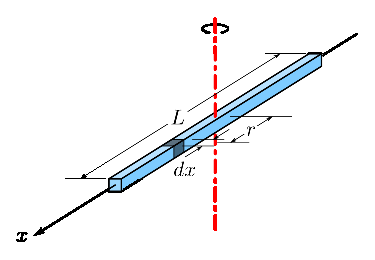
\includegraphics[scale=1.75]{resources/f1.eps}
\end{center}

Dada la ecuación del momento de inercia:

\begin{equation}
    I = \int_{M} r^2\, dm
\label{momentodeinercia1}
\end{equation}

Siendo $r$ equivalente al valor de $|x|$, por tanto:

\begin{equation*}
    r^2 = x^2
\end{equation*}

Asumiendo la distribución homogénea de la masa:

\begin{equation*}
    \lambda = \frac{dm}{dx}
\end{equation*}

Por tanto:

\begin{equation}
    dm = \lambda\, dx
\label{dm1}
\end{equation}

Reemplazando (\ref{dm1}) en (\ref{momentodeinercia1}):

\begin{equation*}
    I = \int_{-L/2}^{L/2} r^2\, \lambda\, dx = \lambda \int_{-L/2}^{L/2} x^2\, dx = \lambda\, \frac{x^3}{3} \Biggr|_{-L/2}^{L/2} = \lambda \left( \frac{(\frac{L}{2})^3}{3} - \frac{(-\frac{L}{2})^3}{3} \right)
\end{equation*}
\begin{equation}
    I = \lambda\, \frac{L^3}{12}
\label{resultado1}
\end{equation}

A partir de la ecuación (\ref{dm1}) sabemos que:

\begin{equation*}
    M = \lambda\, L
\end{equation*}

Despejando $\lambda$ y reemplazando en la ecuación (\ref{resultado1}), obtenemos:

\begin{equation*}
    I = \frac{1}{12} \left( \frac{M}{L} \right) L^3
\end{equation*}

Resultando finalmente:

\begin{equation}
    I = \frac{1}{12}\, M\, L^2
\end{equation}

\newpage
b) Barra uniforme, eje por un extremo y perpendicular a su longitud.

\begin{center}
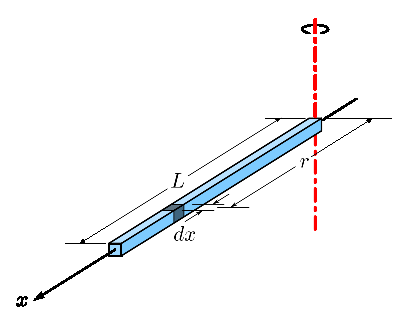
\includegraphics[scale=1.75]{resources/f2.eps}
\end{center}

Dada la ecuación del momento de inercia:

\begin{equation}
    I = \int_{M} r^2\, dm
\label{momentodeinercia2}
\end{equation}

Siendo $r$ equivalente al valor de $|x|$, por tanto:

\begin{equation*}
    r^2 = x^2
\end{equation*}

Asumiendo la distribución homogénea de la masa:

\begin{equation*}
    \lambda = \frac{dm}{dx}
\end{equation*}

Por tanto:

\begin{equation}
    dm = \lambda\, dx
\label{dm2}
\end{equation}

Reemplazando (\ref{dm2}) en (\ref{momentodeinercia2}):

\begin{equation*}
    I = \int_{0}^{L} r^2\, \lambda\, dx = \lambda \int_{0}^{L} x^2\, dx = \lambda\, \frac{x^3}{3} \Biggr|_{0}^{L}
\end{equation*}
\begin{equation}
    I = \lambda\, \frac{L^3}{3}
\label{resultado2}
\end{equation}

A partir de la ecuación (\ref{dm2}) sabemos que:

\begin{equation*}
    M = \lambda\, L
\end{equation*}

Despejando $\lambda$ y reemplazando en la ecuación (\ref{resultado2}), obtenemos:

\begin{equation*}
    I = \frac{1}{3} \left( \frac{M}{L} \right) L^3
\end{equation*}

Resultando finalmente:

\begin{equation}
    I = \frac{1}{3}\, M\, L^2
\end{equation}

\newpage
c) Disco uniforme, eje en el centro de masa y perpendicular al disco.

\begin{center}
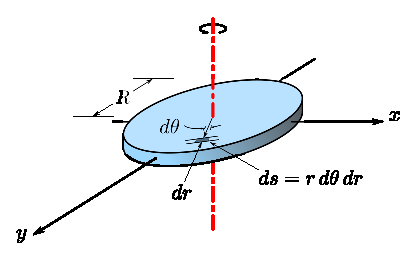
\includegraphics[scale=1.75]{resources/f3.eps}
\end{center}

Dada la ecuación del momento de inercia:

\begin{equation}
    I = \int_{M} r^2\, dm
\label{momentodeinercia3}
\end{equation}

Asumiendo la distribución homogénea de la masa:

\begin{equation*}
    \sigma = \frac{dm}{ds}
\end{equation*}

Usando un diferencial en coordenadas polares obtenemos:

\begin{equation*}
    ds = r\, d\theta\, dr
\end{equation*}

Por tanto:

\begin{equation}
    dm = \sigma\, ds = \sigma\, r\, d\theta\, dr
\label{dm3}
\end{equation}

Reemplazando (\ref{dm3}) en (\ref{momentodeinercia3}):

\begin{equation*}
    I = \int_{S} r^2\, \sigma\, ds = \int_{0}^{R} \int_{0}^{2\pi} r^2\, \sigma\, r\, d\theta\, dr = \sigma \int_{0}^{R} \int_{0}^{2\pi} r^3\, d\theta\, dr = \sigma \int_{0}^{R} ( r^3\, \theta \Biggr|_{0}^{2\pi} )\, dr
\end{equation*}
\begin{equation*}
    I = \sigma \int_{0}^{R} 2\pi\, r^3\, dr = 2\pi\, \sigma \int_{0}^{R} r^3 dr = 2\pi\, \sigma\, \frac{r^4}{4} \Biggr|_{0}^{R} = 2\pi\, \sigma\, \frac{R^4}{4}
\end{equation*}
\begin{equation}
    I = \pi\, \sigma\, \frac{R^4}{2}
\label{resultado3}
\end{equation}

A partir de la ecuación (\ref{dm3}) sabemos que:

\begin{equation*}
    M = \sigma\, S = \sigma\, \pi\, R^2
\end{equation*}

Despejando $\sigma$ y reemplazando en la ecuación (\ref{resultado3}), obtenemos:

\begin{equation*}
    I = \pi\, \left( \frac{M}{\pi\, R^2} \right) \frac{R^4}{2}
\end{equation*}

Resultando finalmente:

\begin{equation}
    I = \frac{1}{2}\, M\, R^2
\end{equation}

\newpage
d) Disco uniforme, eje con el centro de masa y paralelo al disco.

\begin{center}
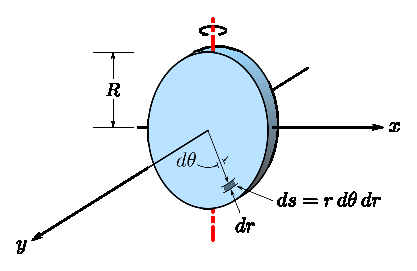
\includegraphics[scale=1.75]{resources/f4.eps}
\end{center}

Dada la ecuación del momento de inercia:

\begin{equation}
    I = \int_{M} r^2\, dm
\label{momentodeinercia4}
\end{equation}

Asumiendo la distribución homogénea de la masa:

\begin{equation*}
    \sigma = \frac{dm}{ds}
\end{equation*}

Usando un diferencial en coordenadas polares obtenemos:

\begin{equation*}
    ds = a\, d\theta\, da
\end{equation*}

Por tanto:

\begin{equation}
    dm = \sigma\, ds = \sigma\, a\, d\theta\, da
\label{dm4}
\end{equation}

Considerando la relación trigonométrica entre las variables $r$ y $a$:

\begin{equation*}
    cos (\theta) = \frac{r}{a}
\end{equation*}

Entonces:

\begin{equation}
    r = a\, cos (\theta)
\label{distancia4}
\end{equation}

Reemplazando (\ref{dm4}) y (\ref{distancia4}) en (\ref{momentodeinercia4}): 

\begin{equation*}
    I = \int_{S} r^2\, \sigma\, ds = \int_{0}^{R} \int_{0}^{2\pi} a^2\, cos^2(\theta)\, \sigma\, a\, d\theta\, da = \sigma \int_{0}^{R} a^3 \int_{0}^{2\pi} cos^2(\theta)\, d\theta\, da
\end{equation*}

Considerando las siguientes propiedades trigonométricas:

\begin{equation*}
    cos^2(x) + sen^2(x) = 1
\end{equation*}
\begin{equation*}
    cos^2(x) - sen^2(x) = cos(2x)
\end{equation*}

Obtenemos:

\begin{equation*}
    2\, cos^2(x) = 1 + cos(2x)
\end{equation*}
\begin{equation}
    cos^2(x) = \frac{1}{2} + \frac{1}{2}\, cos(2x)
\label{trigonometrica4}
\end{equation}

Reemplazando (\ref{trigonometrica4}) en la integral:

\begin{equation*}
    I = \sigma \int_{0}^{R} a^3 \left( \int_{0}^{2\pi} \frac{1}{2} + \frac{1}{2} cos(2\theta) \, d\theta \right) \, da = \sigma \int_{0}^{R} a^3 \left( \frac{1}{2}\, \theta \Biggr|_{0}^{2\pi} + \frac{1}{4} sen(2\theta) \Biggr|_{0}^{2\pi} \right) \, da 
\end{equation*}
\begin{equation*}
    I = \sigma \int_{0}^{R} a^3 \left( \pi + \frac{1}{4} sen(4\pi) - \frac{1}{4} sen(0) \right) \, da = \sigma \int_{0}^{R} a^3 \pi da = \pi\, \sigma \int_{0}^{R} a^3 da = \pi\, \sigma \left( \frac{a^4}{4} \Biggr|_{0}^{R} \right)
\end{equation*}
\begin{equation}
    I = \pi\, \sigma\, \frac{R^4}{4}
\label{resultado4}
\end{equation}

A partir de la ecuación (\ref{dm4}) sabemos que:

\begin{equation*}
    M = \sigma\, S = \sigma\, \pi\, R^2
\end{equation*}

Despejando $\sigma$ y reemplazando en la ecuación (\ref{resultado4}), obtenemos:

\begin{equation*}
    I = \pi\, \left( \frac{M}{\pi\, R^2} \right) \frac{R^4}{4}
\end{equation*}

Resultando finalmente:

\begin{equation}
    I = \frac{1}{4}\, M\, R^2
\end{equation}

\newpage
e) Aro o anillo uniforme, eje en el centro de masa y perpendicular al aro.

\begin{center}
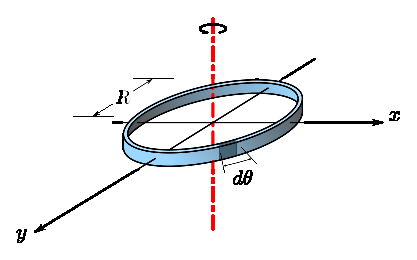
\includegraphics[scale=1.75]{resources/f5.eps}
\end{center}

Dada la ecuación del momento de inercia:

\begin{equation}
    I = \int_{M} r^2\, dm
\label{momentodeinercia5}
\end{equation}

Asumiendo la distribución homogénea de la masa:

\begin{equation*}
    \lambda = \frac{dm}{dl} = \frac{dm}{R\, d\theta}
\end{equation*}

Por tanto:

\begin{equation}
    dm = \lambda\, R\, d\theta
\label{dm5}
\end{equation}

Reemplazando (\ref{dm5}) en (\ref{momentodeinercia5}):

\begin{equation*}
    I = \int_{0}^{2\pi} R^2\, \lambda\, R\, d\theta = R^3\, \lambda\, \int_{0}^{2\pi} d\theta = R^3\, \lambda (\theta \Biggr|_{0}^{2\pi})
\end{equation*}
\begin{equation}
    I = \lambda\, R^3\, 2\pi
\label{resultado5}
\end{equation}

A partir de la ecuación (\ref{dm5}) sabemos que:

\begin{equation*}
    M = \lambda\, l = \lambda\, 2\pi\, R
\end{equation*}

Despejando $\lambda$ y reemplazando en la ecuación (\ref{resultado5}), obtenemos:

\begin{equation*}
    I = \left( \frac{M}{2\pi\, R} \right) R^3\, 2\pi
\end{equation*}

Resultando finalmente:

\begin{equation}
    I = M\, R^2
\end{equation}

\newpage
f) Cilindro macizo uniforme, eje de simetría en el centro de masa.

\begin{center}
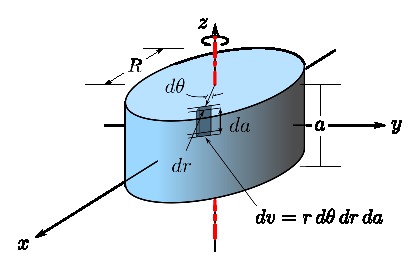
\includegraphics[scale=1.75]{resources/f6.eps}
\end{center}

Dada la ecuación del momento de inercia:

\begin{equation}
    I = \int_{M} r^2\, dm
\label{momentodeinercia6}
\end{equation}

Asumiendo la distribución homogénea de la masa:

\begin{equation*}
    \rho = \frac{dm}{dv} = \frac{dm}{r\, d\theta\, dr\, da}
\end{equation*}

Por tanto:

\begin{equation}
    dm = \rho\, dv = \rho\, r\, d\theta\, dr\, da
\label{dm6}
\end{equation}

Reemplazando (\ref{dm6}) en (\ref{momentodeinercia6}):

\begin{equation*}
    I = \int_{V} r^2\, \rho\, dv = \int_{-a/2}^{a/2} \int_{0}^{R} \int_{0}^{2\pi} r^2\, \rho\, r\, d\theta\, dr\, da = \rho\, \int_{-a/2}^{a/2} \int_{0}^{R} \int_{0}^{2\pi} r^3\, d\theta\, dr\, da
\end{equation*}
\begin{equation*}
    I = \rho\, \int_{-a/2}^{a/2} \int_{0}^{R} (r^3\, \theta \Biggr|_{0}^{2\pi})\, dr\, da = \rho\, \int_{-a/2}^{a/2} \int_{0}^{R} 2\pi\, r^3\, dr\, da = 2\pi\, \rho \int_{-a/2}^{a/2} \left(\frac{r^4}{4}\Biggr|_{0}^{R}\right) da
\end{equation*}
\begin{equation*}
    I = 2\pi\, \rho \int_{-a/2}^{a/2} \frac{R^4}{4}\, da = 2\pi\, \rho \left(\frac{R^4}{4} a\Biggr|_{-a/2}^{a/2}\right) = 2\pi\, \rho\, \left( \frac{R^4}{4} \left( \frac{a}{2} + \frac{a}{2} \right)  \right) = 2\pi\, \rho\, \frac{R^4}{4}\, a
\end{equation*}
\begin{equation}
    I = \frac{1}{2}\, \pi\, \rho\, R^4\, a
\label{resultado6}
\end{equation}

A partir de la ecuación (\ref{dm6}) sabemos que:

\begin{equation*}
    M = \rho\, V = \rho\, \pi\, R^2\, a
\end{equation*}

Despejando $\rho$ y reemplazando en la ecuación (\ref{resultado6}), obtenemos:

\begin{equation*}
    I = \frac{1}{2} \pi\, (\frac{M}{\pi\, R^2\, a})\, R^4\, a
\end{equation*}

Resultando finalmente:

\begin{equation}
    I = \frac{1}{2}\, M\, R^2
\end{equation}

\newpage
g) Esfera maciza uniforme, eje en el centro de masa.

\begin{center}
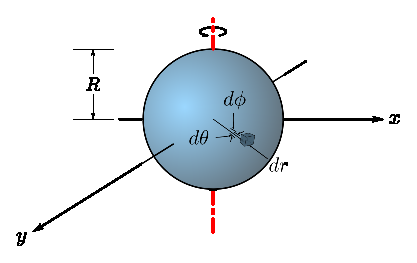
\includegraphics[scale=1.75]{resources/f7.eps}
\end{center}

Dada la ecuación del momento de inercia:

\begin{equation}
    I = \int_{M} r^2\, dm
\label{momentodeinercia7}
\end{equation}

Asumiendo la distribución homogénea de la masa:

\begin{equation*}
    \rho = \frac{dm}{dv}
\end{equation*}

Usando un diferencial en coordenadas esféricas obtenemos:

\begin{equation*}
    dv = da\, a\, d\phi\, a\, sen (\phi)\, d\theta
\end{equation*}
\begin{equation*}
    dv = a^2\, sen (\phi)\, da\, d\phi\, d\theta
\end{equation*}

Por tanto:

\begin{equation}
    dm = \rho\, dv = \rho\, a^2\, sen (\phi)\, da\, d\phi\, d\theta
\label{dm7}
\end{equation}

Considerando la relación trigonométrica entre las variables $r$ y $a$:

\begin{equation}
    r = a\, sen (\phi)
\label{distancia7}
\end{equation}

Reemplazando (\ref{dm7}) y (\ref{distancia7}) en (\ref{momentodeinercia7}): 

\begin{equation*}
    I = \int_{V} r^2\, \rho\, dv = \int_{0}^{2\pi} \int_{0}^{\pi} \int_{0}^{R} a^2\, sen^2(\phi)\, \rho\, a^2\, sen (\phi)\, da\, d\phi\, d\theta
\end{equation*}
\begin{equation*}
    I = \rho\, \int_{0}^{2\pi} \int_{0}^{\pi} \int_{0}^{R} a^4\, sen^3(\phi)\, da\, d\phi\, d\theta = \rho\, \int_{0}^{2\pi} \int_{0}^{\pi} \left(\frac{a^5}{5}\Biggr|_{0}^{R}\right)\, sen^3(\phi)\, d\phi\, d\theta
\end{equation*}
\begin{equation*}
    I = \rho\, \int_{0}^{2\pi} \int_{0}^{\pi} \frac{R^5}{5}\, sen^3(\phi)\, d\phi\, d\theta = \rho\, \frac{R^5}{5}\, \int_{0}^{2\pi} \int_{0}^{\pi} sen^3(\phi)\, d\phi\, d\theta
\end{equation*}
\begin{equation*}
    I = \rho\, \frac{R^5}{5}\, \int_{0}^{2\pi} \int_{0}^{\pi} sen^2(\phi)\, sen(\phi)\, d\phi\, d\theta = \rho\, \frac{R^5}{5}\, \int_{0}^{2\pi} \int_{0}^{\pi} (1 - cos^2(\phi))\, sen(\phi)\, d\phi\, d\theta
\end{equation*}
\begin{equation*}
    I = \rho\, \frac{R^5}{5}\, \int_{0}^{2\pi} \left( \int_{0}^{\pi} sen(\phi)\, d\phi - \int_{0}^{\pi} cos^2(\phi)\, sen(\phi)\, d\phi\, \right) d\theta
\end{equation*}
\begin{equation*}
    I = \rho\, \frac{R^5}{5}\, \int_{0}^{2\pi} \left( -cos(\phi)\Biggr|_{0}^{\pi} + \frac{cos^3(\phi)}{3}\Biggr|_{0}^{\pi} \right) d\theta
\end{equation*}
\begin{equation*}
    I = \rho\, \frac{R^5}{5}\, \int_{0}^{2\pi} \left( -cos(\pi) + cos(0) + \frac{cos^3(\pi)}{3} - \frac{cos^3(0)}{3} \right) d\theta
\end{equation*}
\begin{equation*}
    I = \rho\, \frac{R^5}{5}\, \int_{0}^{2\pi} \left( 1 + 1 - \frac{1}{3} - \frac{1}{3} \right) d\theta = \rho\, \frac{R^5}{5}\, \int_{0}^{2\pi} \frac{4}{3} d\theta = \rho\, \frac{4\, R^5}{15} \int_{0}^{2\pi} d\theta = \rho\, \frac{4\, R^5}{15} ( \theta \Biggr|_{0}^{2\pi} )
\end{equation*}
\begin{equation}
    I = \rho\, \frac{8\pi}{15}\, R^5
\label{resultado7}
\end{equation}

A partir de la ecuación (\ref{dm7}) sabemos que:

\begin{equation*}
    M = \rho\, V = \rho\, \frac{4\pi}{3} R^3
\end{equation*}

Despejando $\rho$ y reemplazando en la ecuación (\ref{resultado7}), obtenemos:

\begin{equation*}
    I = (\frac{3\, M}{4\pi\, R^3})\, \frac{8\pi\, R^5}{15}
\end{equation*}

Resultando finalmente:

\begin{equation}
    I = \frac{2}{5}\, M\, R^2
\end{equation}

\newpage
h) Cascarón esférico uniforme, eje en el centro de masa.

\begin{center}
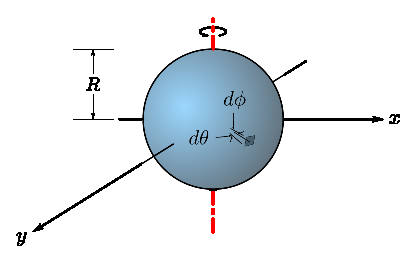
\includegraphics[scale=1.75]{resources/f8.eps}
\end{center}

Dada la ecuación del momento de inercia:

\begin{equation}
    I = \int_{M} r^2\, dm
\label{momentodeinercia8}
\end{equation}

Asumiendo la distribución homogénea de la masa:

\begin{equation*}
    \sigma = \frac{dm}{ds}
\end{equation*}

Usando un diferencial en coordenadas esféricas obtenemos:

\begin{equation*}
    ds = R\, d\phi\, R\, sen(\phi)\, d\theta
\end{equation*}
\begin{equation*}
    ds = R^2\, sen (\phi)\, d\phi\, d\theta
\end{equation*}

Por tanto:

\begin{equation}
    dm = \sigma\, ds = \sigma\, R^2\, sen (\phi)\, d\phi\, d\theta
\label{dm8}
\end{equation}

Considerando la relación trigonométrica entre las variables $r$ y $R$:

\begin{equation}
    r = R\, sen (\phi)
\label{distancia8}
\end{equation}

Reemplazando (\ref{dm8}) y (\ref{distancia8}) en (\ref{momentodeinercia8}): 

\begin{equation*}
    I = \int_{S} r^2\, \sigma\, ds = \int_{0}^{2\pi} \int_{0}^{\pi} R^2\, sen^2(\phi)\, \sigma\, R^2\, sen (\phi)\, d\phi\, d\theta = \int_{0}^{2\pi} \int_{0}^{\pi} \sigma R^4\, sen^3(\phi)\, d\phi\, d\theta
\end{equation*}
\begin{equation*}
    I = \sigma\, R^4\, \int_{0}^{2\pi} \int_{0}^{\pi}\, sen^3(\phi)\, d\phi\, d\theta = \sigma\, R^4\, \int_{0}^{2\pi} \int_{0}^{\pi} sen^2(\phi)\, sen(\phi)\, d\phi\, d\theta
\end{equation*}
\begin{equation*}
    I = \sigma\, R^4\, \int_{0}^{2\pi} \int_{0}^{\pi} (1 - cos^2(\phi))\, sen(\phi)\, d\phi\, d\theta
\end{equation*}
\begin{equation*}
    I = \sigma\, R^4\, \int_{0}^{2\pi} \left( \int_{0}^{\pi} sen(\phi)\, d\phi - \int_{0}^{\pi} cos^2(\phi)\, sen(\phi)\, d\phi\, \right) d\theta
\end{equation*}
\begin{equation*}
    I = \sigma\, R^4\, \int_{0}^{2\pi} \left( -cos(\phi)\Biggr|_{0}^{\pi} + \frac{cos^3(\phi)}{3}\Biggr|_{0}^{\pi} \right) d\theta
\end{equation*}
\begin{equation*}
    I = \sigma\, R^4\, \int_{0}^{2\pi} \left( -cos(\pi) + cos(0) + \frac{cos^3(\pi)}{3} - \frac{cos^3(0)}{3} \right) d\theta
\end{equation*}
\begin{equation*}
    I = \sigma\, R^4\, \int_{0}^{2\pi} \left( 1 + 1 - \frac{1}{3} - \frac{1}{3} \right) d\theta = \sigma\, R^4\, \int_{0}^{2\pi} \frac{4}{3} d\theta = \sigma\, \frac{4\, R^4}{3} \int_{0}^{2\pi} d\theta = \sigma\, \frac{4\, R^4}{3} ( \theta \Biggr|_{0}^{2\pi} )
\end{equation*}
\begin{equation}
    I = \sigma\, \frac{8\pi}{3} R^4
\label{resultado8}
\end{equation}

A partir de la ecuación (\ref{dm8}) sabemos que:

\begin{equation*}
    M = \sigma\, S = \sigma\, 4\pi\, R^2
\end{equation*}

Despejando $\sigma$ y reemplazando en la ecuación (\ref{resultado8}), obtenemos:

\begin{equation*}
    I = (\frac{M}{4\pi\, R^2})\, \frac{8\pi\, R^4}{3}
\end{equation*}

Resultando finalmente:

\begin{equation}
    I = \frac{2}{3}\, M\, R^2
\end{equation}

\end{document}

